\documentclass{beamer}
\setbeamertemplate{caption}[numbered]
\usepackage{tikz}
\usepackage{graphicx}
\usetheme{AnnArbor}
%\usecolortheme{wolverine}
\title[AD for POMPs]{Automatic Differentiation Accelerates Inference for Partially Observed Stochastic Processes}
\author[Kevin Tan]{Kevin Tan \\ \small{University of Pennsylvania, Department of Statistics and Data Science\\\vspace{0.5cm} \small{Advised by Giles Hooker and Edward Ionides}}}


\usepackage{amsmath}
\usepackage{tabularx}
\usepackage{mathtools}
\usepackage{bbold}
\usepackage[utf8]{inputenc} % allow utf-8 input
\usepackage[T1]{fontenc}    % use 8-bit T1 fonts
\usepackage{pifont}
%\usepackage[left=1in,right=1in,]{geometry}
\usepackage{multicol,lipsum,xcolor}
\usepackage{hyperref}       % hyperlinks
\usepackage{url}            % simple URL typesetting
\usepackage{amsmath,amsthm,amssymb,bm}
\usepackage{bbold}
\usepackage{caption}
\usepackage{graphicx}
\usepackage{enumerate}
%\usepackage{enumitem}
\usepackage{natbib}
\usepackage{parskip}
\usepackage{comment}
\usepackage{microtype}
\usepackage{diagbox}
\usepackage{tikz}
\usepackage{fancyhdr}
\usepackage{appendixnumberbeamer}


\newcommand{\Prob}{\displaystyle \mathbb {P}}
\newcommand{\jac}{\bigg| \frac{\dif x}{\dif y} \bigg|}
\newcommand{\inftyint}{\int_{-\infty}^{\infty}}
\newcommand{\X}{\mathcal{X}}
\newcommand{\Y}{\mathcal{Y}}
\newcommand{\N}{\mathbb{N}}
\newcommand{\Z}{\mathbb{Z}}
\newcommand{\C}{\mathbb{C}}

% best package ever
%\usepackage{realhats}

\def\mathfamilydefault{\rmdefault}

\usepackage{color}
\usepackage{xcolor}
\definecolor{hlpink}{rgb}{0.96, 0.76, 0.76}
\definecolor{hlblue}{rgb}{0.54, 0.81, 0.94}
\definecolor{hlyellow}{rgb}{0.98, 0.91, 0.71}
\definecolor{hlgreen}{rgb}{0.7, 0.93, 0.36}
\definecolor{hlpurple}{rgb}{0.8, 0.8, 1.0}

\newcommand{\highlight}[2][yellow]{\mathchoice%
  {\colorbox{#1}{$\displaystyle#2$}}%
  {\colorbox{#1}{$\textstyle#2$}}%
  {\colorbox{#1}{$\scriptstyle#2$}}%
  {\colorbox{#1}{$\scriptscriptstyle#2$}}}%
  
 \AtBeginSection[]{
  \begin{frame}
  \vfill
  \centering
  \begin{beamercolorbox}[sep=8pt,center,shadow=true,rounded=true]{title}
    \usebeamerfont{title}\insertsectionhead\par%
  \end{beamercolorbox}
  \vfill
  \end{frame}
}


%%%%% NEW MATH DEFINITIONS %%%%%
\usepackage{amsmath,bbm,bm}
\usepackage{amsfonts}
\usepackage{amsthm}
\usepackage{mathtools}

% algorithm
\usepackage{algorithm, algorithmic}
\usepackage{tabularx}
%\usepackage[table,xcdraw]{xcolor}
\usepackage{xcolor}
% commands
% global count (no section number)
\newtheorem{thm}{Theorem}%[section]
\newtheorem{lem}{Lemma}
\newtheorem{prop}{Proposition}
\newtheorem{cor}{Corollary}
\newtheorem{conj}{Conjecture}
\newtheorem{aspt}{Assumption}
\newtheorem{claim}{Claim}
\newtheorem{rmk}{Remark}
\newtheorem{commt}{Comment}
\newtheorem{defn}{Definition}

% Comments
% \usepackage{xcolor} % already loaded
\newcount\comments  % 0 suppresses notes to selves in text
\comments=0  % TODO: change to 0 for final version
\newcommand{\genComment}[2]{\ifnum\comments=1{\textcolor{#1}{\textsf{\footnotesize #2}}}\fi}
\newcommand{\ed}[1]{\genComment{red}{[EI:#1]}}
\newcommand{\giles}[1]{\genComment{green}{[GH:#1]}}
\newcommand{\kevin}[1]{\genComment{blue}{[KT:#1]}}

% Mark sections of captions for referring to divisions of figures
\newcommand{\figleft}{{\em (Left)}}
\newcommand{\figcenter}{{\em (Center)}}
\newcommand{\figright}{{\em (Right)}}
\newcommand{\figtop}{{\em (Top)}}
\newcommand{\figbottom}{{\em (Bottom)}}
\newcommand{\captiona}{{\em (a)}}
\newcommand{\captionb}{{\em (b)}}
\newcommand{\captionc}{{\em (c)}}
\newcommand{\captiond}{{\em (d)}}


\newcommand\seq[2]{{#1}\!:\!{#2}}
\newcommand\R{\mathbb{R}}
\newcommand\Var{\mathrm{Var}}
\newcommand\var{\Var}
\newcommand\Cov{\mathrm{Cov}}
\newcommand\cov{\Cov}
\newcommand\iid{\mathrm{iid}}
\newcommand\dist{d}
\newcommand\lik{\mathcal{L}}
\newcommand\prob{\mathbb{P}}
\newcommand\E{\mathbb{E}}
\newcommand\loglik{\ell}
\newcommand\process{\texttt{process}}
\newcommand\dimtheta{\mathrm{dim}_{\Theta}}
\newcommand\param{\,;}
\newcommand\giventh\param
\newcommand\given{{\,\vert\,}}
\newcommand\code[1]{\texttt{#1}}

\renewcommand\time{n}
\newcommand\myvec[1]{\boldsymbol{#1}}
\newcommand\altTime{\tilde n}
\newcommand\Time{N}
\newcommand\Np{J}
\newcommand\np{j}
\newcommand\altNp{k}
\newcommand\altAltNp{\tilde j}
\newcommand\resampleIndex{r}

% color
\newcommand{\blue}[1]{\textcolor{blue}{#1}}
\newcommand{\red}[1]{\textcolor{red}{#1}}
\newcommand{\orange}[1]{\textcolor{orange}{#1}}
\newcommand{\green}[1]{\textcolor{green}{#1}}

% Highlight a newly defined term
\newcommand{\newterm}[1]{{\bf #1}}


% Figure reference, lower-case.
\def\figref#1{figure~\ref{#1}}
% Figure reference, capital. For start of sentence
\def\Figref#1{Figure~\ref{#1}}
\def\twofigref#1#2{figures \ref{#1} and \ref{#2}}
\def\quadfigref#1#2#3#4{figures \ref{#1}, \ref{#2}, \ref{#3} and \ref{#4}}
% Section reference, lower-case.
\def\secref#1{section~\ref{#1}}
% Section reference, capital.
\def\Secref#1{Section~\ref{#1}}
% Reference to two sections.
\def\twosecrefs#1#2{sections \ref{#1} and \ref{#2}}
% Reference to three sections.
\def\secrefs#1#2#3{sections \ref{#1}, \ref{#2} and \ref{#3}}
% Reference to an equation, lower-case.
\def\eqref#1{equation~\ref{#1}}
% Reference to an equation, upper case
\def\Eqref#1{Equation~\ref{#1}}
% A raw reference to an equation---avoid using if possible
\def\plaineqref#1{\ref{#1}}
% Reference to a chapter, lower-case.
\def\chapref#1{chapter~\ref{#1}}
% Reference to an equation, upper case.
\def\Chapref#1{Chapter~\ref{#1}}
% Reference to a range of chapters
\def\rangechapref#1#2{chapters\ref{#1}--\ref{#2}}
% Reference to an algorithm, lower-case.
\def\algref#1{algorithm~\ref{#1}}
% Reference to an algorithm, upper case.
\def\Algref#1{Algorithm~\ref{#1}}
\def\twoalgref#1#2{algorithms \ref{#1} and \ref{#2}}
\def\Twoalgref#1#2{Algorithms \ref{#1} and \ref{#2}}
% Reference to a part, lower case
\def\partref#1{part~\ref{#1}}
% Reference to a part, upper case
\def\Partref#1{Part~\ref{#1}}
\def\twopartref#1#2{parts \ref{#1} and \ref{#2}}

\def\ceil#1{\lceil #1 \rceil}
\def\floor#1{\lfloor #1 \rfloor}
\def\1{\bm{1}}
\newcommand{\train}{\mathcal{D}}
\newcommand{\valid}{\mathcal{D_{\mathrm{valid}}}}
\newcommand{\test}{\mathcal{D_{\mathrm{test}}}}

\def\eps{{\epsilon}}


% Random variables
\def\reta{{\textnormal{$\eta$}}}
\def\ra{{\textnormal{a}}}
\def\rb{{\textnormal{b}}}
\def\rc{{\textnormal{c}}}
\def\rd{{\textnormal{d}}}
\def\re{{\textnormal{e}}}
\def\rf{{\textnormal{f}}}
\def\rg{{\textnormal{g}}}
\def\rh{{\textnormal{h}}}
\def\ri{{\textnormal{i}}}
\def\rj{{\textnormal{j}}}
\def\rk{{\textnormal{k}}}
\def\rl{{\textnormal{l}}}
% rm is already a command, just don't name any random variables m
\def\rn{{\textnormal{n}}}
\def\ro{{\textnormal{o}}}
\def\rp{{\textnormal{p}}}
\def\rq{{\textnormal{q}}}
\def\rr{{\textnormal{r}}}
\def\rs{{\textnormal{s}}}
\def\rt{{\textnormal{t}}}
\def\ru{{\textnormal{u}}}
\def\rv{{\textnormal{v}}}
\def\rw{{\textnormal{w}}}
\def\rx{{\textnormal{x}}}
\def\ry{{\textnormal{y}}}
\def\rz{{\textnormal{z}}}

% Random vectors
\def\rvepsilon{{\mathbf{\epsilon}}}
\def\rvtheta{{\mathbf{\theta}}}
\def\rva{{\mathbf{a}}}
\def\rvb{{\mathbf{b}}}
\def\rvc{{\mathbf{c}}}
\def\rvd{{\mathbf{d}}}
\def\rve{{\mathbf{e}}}
\def\rvf{{\mathbf{f}}}
\def\rvg{{\mathbf{g}}}
\def\rvh{{\mathbf{h}}}
\def\rvu{{\mathbf{i}}}
\def\rvj{{\mathbf{j}}}
\def\rvk{{\mathbf{k}}}
\def\rvl{{\mathbf{l}}}
\def\rvm{{\mathbf{m}}}
\def\rvn{{\mathbf{n}}}
\def\rvo{{\mathbf{o}}}
\def\rvp{{\mathbf{p}}}
\def\rvq{{\mathbf{q}}}
\def\rvr{{\mathbf{r}}}
\def\rvs{{\mathbf{s}}}
\def\rvt{{\mathbf{t}}}
\def\rvu{{\mathbf{u}}}
\def\rvv{{\mathbf{v}}}
\def\rvw{{\mathbf{w}}}
\def\rvx{{\mathbf{x}}}
\def\rvy{{\mathbf{y}}}
\def\rvz{{\mathbf{z}}}

% Elements of random vectors
\def\erva{{\textnormal{a}}}
\def\ervb{{\textnormal{b}}}
\def\ervc{{\textnormal{c}}}
\def\ervd{{\textnormal{d}}}
\def\erve{{\textnormal{e}}}
\def\ervf{{\textnormal{f}}}
\def\ervg{{\textnormal{g}}}
\def\ervh{{\textnormal{h}}}
\def\ervi{{\textnormal{i}}}
\def\ervj{{\textnormal{j}}}
\def\ervk{{\textnormal{k}}}
\def\ervl{{\textnormal{l}}}
\def\ervm{{\textnormal{m}}}
\def\ervn{{\textnormal{n}}}
\def\ervo{{\textnormal{o}}}
\def\ervp{{\textnormal{p}}}
\def\ervq{{\textnormal{q}}}
\def\ervr{{\textnormal{r}}}
\def\ervs{{\textnormal{s}}}
\def\ervt{{\textnormal{t}}}
\def\ervu{{\textnormal{u}}}
\def\ervv{{\textnormal{v}}}
\def\ervw{{\textnormal{w}}}
\def\ervx{{\textnormal{x}}}
\def\ervy{{\textnormal{y}}}
\def\ervz{{\textnormal{z}}}

% Random matrices
\def\rmA{{\mathbf{A}}}
\def\rmB{{\mathbf{B}}}
\def\rmC{{\mathbf{C}}}
\def\rmD{{\mathbf{D}}}
\def\rmE{{\mathbf{E}}}
\def\rmF{{\mathbf{F}}}
\def\rmG{{\mathbf{G}}}
\def\rmH{{\mathbf{H}}}
\def\rmI{{\mathbf{I}}}
\def\rmJ{{\mathbf{J}}}
\def\rmK{{\mathbf{K}}}
\def\rmL{{\mathbf{L}}}
\def\rmM{{\mathbf{M}}}
\def\rmN{{\mathbf{N}}}
\def\rmO{{\mathbf{O}}}
\def\rmP{{\mathbf{P}}}
\def\rmQ{{\mathbf{Q}}}
\def\rmR{{\mathbf{R}}}
\def\rmS{{\mathbf{S}}}
\def\rmT{{\mathbf{T}}}
\def\rmU{{\mathbf{U}}}
\def\rmV{{\mathbf{V}}}
\def\rmW{{\mathbf{W}}}
\def\rmX{{\mathbf{X}}}
\def\rmY{{\mathbf{Y}}}
\def\rmZ{{\mathbf{Z}}}

% Elements of random matrices
\def\ermA{{\textnormal{A}}}
\def\ermB{{\textnormal{B}}}
\def\ermC{{\textnormal{C}}}
\def\ermD{{\textnormal{D}}}
\def\ermE{{\textnormal{E}}}
\def\ermF{{\textnormal{F}}}
\def\ermG{{\textnormal{G}}}
\def\ermH{{\textnormal{H}}}
\def\ermI{{\textnormal{I}}}
\def\ermJ{{\textnormal{J}}}
\def\ermK{{\textnormal{K}}}
\def\ermL{{\textnormal{L}}}
\def\ermM{{\textnormal{M}}}
\def\ermN{{\textnormal{N}}}
\def\ermO{{\textnormal{O}}}
\def\ermP{{\textnormal{P}}}
\def\ermQ{{\textnormal{Q}}}
\def\ermR{{\textnormal{R}}}
\def\ermS{{\textnormal{S}}}
\def\ermT{{\textnormal{T}}}
\def\ermU{{\textnormal{U}}}
\def\ermV{{\textnormal{V}}}
\def\ermW{{\textnormal{W}}}
\def\ermX{{\textnormal{X}}}
\def\ermY{{\textnormal{Y}}}
\def\ermZ{{\textnormal{Z}}}

% Vectors
\def\vzero{{\bm{0}}}
\def\vone{{\bm{1}}}
\def\vmu{{\bm{\mu}}}
\def\vtheta{{\bm{\theta}}}
\def\va{{\bm{a}}}
\def\vb{{\bm{b}}}
\def\vc{{\bm{c}}}
\def\vd{{\bm{d}}}
\def\ve{{\bm{e}}}
\def\vf{{\bm{f}}}
\def\vg{{\bm{g}}}
\def\vh{{\bm{h}}}
\def\vi{{\bm{i}}}
\def\vj{{\bm{j}}}
\def\vk{{\bm{k}}}
\def\vl{{\bm{l}}}
\def\vm{{\bm{m}}}
\def\vn{{\bm{n}}}
\def\vo{{\bm{o}}}
\def\vp{{\bm{p}}}
\def\vq{{\bm{q}}}
\def\vr{{\bm{r}}}
\def\vs{{\bm{s}}}
\def\vt{{\bm{t}}}
\def\vu{{\bm{u}}}
\def\vv{{\bm{v}}}
\def\vw{{\bm{w}}}
\def\vx{{\bm{x}}}
\def\vy{{\bm{y}}}
\def\vz{{\bm{z}}}

% Elements of vectors
\def\evalpha{{\alpha}}
\def\evbeta{{\beta}}
\def\evepsilon{{\epsilon}}
\def\evlambda{{\lambda}}
\def\evomega{{\omega}}
\def\evmu{{\mu}}
\def\evpsi{{\psi}}
\def\evsigma{{\sigma}}
\def\evtheta{{\theta}}
\def\eva{{a}}
\def\evb{{b}}
\def\evc{{c}}
\def\evd{{d}}
\def\eve{{e}}
\def\evf{{f}}
\def\evg{{g}}
\def\evh{{h}}
\def\evi{{i}}
\def\evj{{j}}
\def\evk{{k}}
\def\evl{{l}}
\def\evm{{m}}
\def\evn{{n}}
\def\evo{{o}}
\def\evp{{p}}
\def\evq{{q}}
\def\evr{{r}}
\def\evs{{s}}
\def\evt{{t}}
\def\evu{{u}}
\def\evv{{v}}
\def\evw{{w}}
\def\evx{{x}}
\def\evy{{y}}
\def\evz{{z}}

% Matrix
\def\mA{{\bm{A}}}
\def\mB{{\bm{B}}}
\def\mC{{\bm{C}}}
\def\mD{{\bm{D}}}
\def\mE{{\bm{E}}}
\def\mF{{\bm{F}}}
\def\mG{{\bm{G}}}
\def\mH{{\bm{H}}}
\def\mI{{\bm{I}}}
\def\mJ{{\bm{J}}}
\def\mK{{\bm{K}}}
\def\mL{{\bm{L}}}
\def\mM{{\bm{M}}}
\def\mN{{\bm{N}}}
\def\mO{{\bm{O}}}
\def\mP{{\bm{P}}}
\def\mQ{{\bm{Q}}}
\def\mR{{\bm{R}}}
\def\mS{{\bm{S}}}
\def\mT{{\bm{T}}}
\def\mU{{\bm{U}}}
\def\mV{{\bm{V}}}
\def\mW{{\bm{W}}}
\def\mX{{\bm{X}}}
\def\mY{{\bm{Y}}}
\def\mZ{{\bm{Z}}}
\def\mBeta{{\bm{\beta}}}
\def\mPhi{{\bm{\Phi}}}
\def\mLambda{{\bm{\Lambda}}}
\def\mSigma{{\bm{\Sigma}}}

% Tensor
\DeclareMathAlphabet{\mathsfit}{\encodingdefault}{\sfdefault}{m}{sl}
\SetMathAlphabet{\mathsfit}{bold}{\encodingdefault}{\sfdefault}{bx}{n}
\newcommand{\tens}[1]{\bm{\mathsfit{#1}}}
\def\tA{{\tens{A}}}
\def\tB{{\tens{B}}}
\def\tC{{\tens{C}}}
\def\tD{{\tens{D}}}
\def\tE{{\tens{E}}}
\def\tF{{\tens{F}}}
\def\tG{{\tens{G}}}
\def\tH{{\tens{H}}}
\def\tI{{\tens{I}}}
\def\tJ{{\tens{J}}}
\def\tK{{\tens{K}}}
\def\tL{{\tens{L}}}
\def\tM{{\tens{M}}}
\def\tN{{\tens{N}}}
\def\tO{{\tens{O}}}
\def\tP{{\tens{P}}}
\def\tQ{{\tens{Q}}}
\def\tR{{\tens{R}}}
\def\tS{{\tens{S}}}
\def\tT{{\tens{T}}}
\def\tU{{\tens{U}}}
\def\tV{{\tens{V}}}
\def\tW{{\tens{W}}}
\def\tX{{\tens{X}}}
\def\tY{{\tens{Y}}}
\def\tZ{{\tens{Z}}}


% Graph
\def\gA{{\mathcal{A}}}
\def\gB{{\mathcal{B}}}
\def\gC{{\mathcal{C}}}
\def\gD{{\mathcal{D}}}
\def\gE{{\mathcal{E}}}
\def\gF{{\mathcal{F}}}
\def\gG{{\mathcal{G}}}
\def\gH{{\mathcal{H}}}
\def\gI{{\mathcal{I}}}
\def\gJ{{\mathcal{J}}}
\def\gK{{\mathcal{K}}}
\def\gL{{\mathcal{L}}}
\def\gM{{\mathcal{M}}}
\def\gN{{\mathcal{N}}}
\def\gO{{\mathcal{O}}}
\def\gP{{\mathcal{P}}}
\def\gQ{{\mathcal{Q}}}
\def\gR{{\mathcal{R}}}
\def\gS{{\mathcal{S}}}
\def\gT{{\mathcal{T}}}
\def\gU{{\mathcal{U}}}
\def\gV{{\mathcal{V}}}
\def\gW{{\mathcal{W}}}
\def\gX{{\mathcal{X}}}
\def\gY{{\mathcal{Y}}}
\def\gZ{{\mathcal{Z}}}

% Sets
\def\sA{{\mathbb{A}}}
\def\sB{{\mathbb{B}}}
\def\sC{{\mathbb{C}}}
\def\sD{{\mathbb{D}}}
% Don't use a set called E, because this would be the same as our symbol
% for expectation.
\def\sF{{\mathbb{F}}}
\def\sG{{\mathbb{G}}}
\def\sH{{\mathbb{H}}}
\def\sI{{\mathbb{I}}}
\def\sJ{{\mathbb{J}}}
\def\sK{{\mathbb{K}}}
\def\sL{{\mathbb{L}}}
\def\sM{{\mathbb{M}}}
\def\sN{{\mathbb{N}}}
\def\sO{{\mathbb{O}}}
\def\sP{{\mathbb{P}}}
\def\sQ{{\mathbb{Q}}}
\def\sR{{\mathbb{R}}}
\def\sS{{\mathbb{S}}}
\def\sT{{\mathbb{T}}}
\def\sU{{\mathbb{U}}}
\def\sV{{\mathbb{V}}}
\def\sW{{\mathbb{W}}}
\def\sX{{\mathbb{X}}}
\def\sY{{\mathbb{Y}}}
\def\sZ{{\mathbb{Z}}}

% Entries of a matrix
\def\emLambda{{\Lambda}}
\def\emA{{A}}
\def\emB{{B}}
\def\emC{{C}}
\def\emD{{D}}
\def\emE{{E}}
\def\emF{{F}}
\def\emG{{G}}
\def\emH{{H}}
\def\emI{{I}}
\def\emJ{{J}}
\def\emK{{K}}
\def\emL{{L}}
\def\emM{{M}}
\def\emN{{N}}
\def\emO{{O}}
\def\emP{{P}}
\def\emQ{{Q}}
\def\emR{{R}}
\def\emS{{S}}
\def\emT{{T}}
\def\emU{{U}}
\def\emV{{V}}
\def\emW{{W}}
\def\emX{{X}}
\def\emY{{Y}}
\def\emZ{{Z}}
\def\emSigma{{\Sigma}}

% entries of a tensor
% Same font as tensor, without \bm wrapper
\newcommand{\etens}[1]{\mathsfit{#1}}
\def\etLambda{{\etens{\Lambda}}}
\def\etA{{\etens{A}}}
\def\etB{{\etens{B}}}
\def\etC{{\etens{C}}}
\def\etD{{\etens{D}}}
\def\etE{{\etens{E}}}
\def\etF{{\etens{F}}}
\def\etG{{\etens{G}}}
\def\etH{{\etens{H}}}
\def\etI{{\etens{I}}}
\def\etJ{{\etens{J}}}
\def\etK{{\etens{K}}}
\def\etL{{\etens{L}}}
\def\etM{{\etens{M}}}
\def\etN{{\etens{N}}}
\def\etO{{\etens{O}}}
\def\etP{{\etens{P}}}
\def\etQ{{\etens{Q}}}
\def\etR{{\etens{R}}}
\def\etS{{\etens{S}}}
\def\etT{{\etens{T}}}
\def\etU{{\etens{U}}}
\def\etV{{\etens{V}}}
\def\etW{{\etens{W}}}
\def\etX{{\etens{X}}}
\def\etY{{\etens{Y}}}
\def\etZ{{\etens{Z}}}

% The true underlying data generating distribution
\newcommand{\pdata}{p_{\rm{data}}}
% The empirical distribution defined by the training set
\newcommand{\ptrain}{\hat{p}_{\rm{data}}}
\newcommand{\Ptrain}{\hat{P}_{\rm{data}}}
% The model distribution
\newcommand{\pmodel}{p_{\rm{model}}}
\newcommand{\Pmodel}{P_{\rm{model}}}
\newcommand{\ptildemodel}{\tilde{p}_{\rm{model}}}
% Stochastic autoencoder distributions
\newcommand{\pencode}{p_{\rm{encoder}}}
\newcommand{\pdecode}{p_{\rm{decoder}}}
\newcommand{\precons}{p_{\rm{reconstruct}}}

\newcommand{\laplace}{\mathrm{Laplace}} % Laplace distribution

\newcommand{\Ls}{\mathcal{L}}
\newcommand{\emp}{\tilde{p}}
\newcommand{\lr}{\alpha}
\newcommand{\reg}{\lambda}
\newcommand{\rect}{\mathrm{rectifier}}
\newcommand{\softmax}{\mathrm{softmax}}
\newcommand{\sigmoid}{\sigma}
\newcommand{\softplus}{\zeta}
\newcommand{\KL}{D_{\mathrm{KL}}}
%\newcommand{\Var}{\mathrm{Var}}
\newcommand{\standarderror}{\mathrm{SE}}
%\newcommand{\Cov}{\mathrm{Cov}}
% Wolfram Mathworld says $L^2$ is for function spaces and $\ell^2$ is for vectors
% But then they seem to use $L^2$ for vectors throughout the site, and so does
% wikipedia.
\newcommand{\normlzero}{L^0}
\newcommand{\normlone}{L^1}
\newcommand{\normltwo}{L^2}
\newcommand{\normlp}{L^p}
\newcommand{\normmax}{L^\infty}

\newcommand{\parents}{Pa} % See usage in notation.tex. Chosen to match Daphne's book.

\let\ab\allowbreak

  
\begin{document}



\maketitle


\section{Background}


\begin{frame}{Partially Observed Markov Processes}

    \begin{itemize}
        \item Unobserved Markov process $\{X_t, t \geq t_0\}$, observations $Y_1,...,Y_N \in \gY$ taking values $y_1^*,...,y_N^*$ at timesteps $t_1,..., t_N$. Write $X_n := X_{t_n} \subseteq \R^d$.
        \item \pause Unknown parameter $\theta \in \Theta \subseteq \R^p$, to be estimated.
        \item \textbf{Notation:}
        \begin{itemize}
            \item $f_{X_n|X_{n-1}}\left(x_{n} \mid x_{n-1}; \theta\right)$ is the \textbf{process model}.
            \item \pause $\texttt{process}\left(x_n, \theta\right)$ is the \textbf{simulator} corresponding to the process model. 
            \item \pause $f_{Y_n|X_n}\left(y_n \mid x_n, \theta\right)$ is the \textbf{measurement model}.
        \end{itemize}
    \end{itemize}
\end{frame}


\begin{frame}{Partially Observed Markov Processes}

    
\begin{figure}[H]
\centering
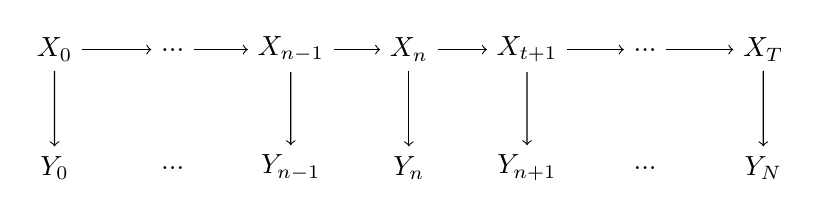
\begin{tikzpicture}[scale=1.5]

\node[black] (X_0) at (-3,0) {$X_0$};
\node[black] (Xdot0) at (-2,0) {$...$};
\node[black] (X_{n-1}) at (-1,0) {$X_{n-1}$};
\node[black] (X_n) at (0,0) {$X_n$};
\node[black] (X_{n+1}) at (1,0) {$X_{t+1}$};
\node[black] (Xdot{n+1}) at (2,0) {$...$};
\node[black] (X_N) at (3,0) {$X_T$};
\node[black] (Y_0) at (-3,-1) {$Y_0$};
\node[black] (Ydot0) at (-2,-1) {$...$};
\node[black] (Y_{n-1}) at (-1,-1) {$Y_{n-1}$};
\node[black] (Y_n) at (-0,-1) {$Y_n$};
\node[black] (Y_{n+1}) at (1,-1) {$Y_{n+1}$};
\node[black] (Ydot{n+1}) at (2,-1) {$...$};
\node[black] (Y_N) at (3,-1) {$Y_N$};
\path[->, black] (X_0) edge (Xdot0);
\path[->, black] (Xdot0) edge (X_{n-1});
\path[->, black] (X_{n-1}) edge (X_n);
\path[->, black] (X_n) edge (X_{n+1});
\path[->, black] (X_{n+1}) edge (Xdot{n+1});
\path[->, black] (Xdot{n+1}) edge (X_N);
\path[->, black] (X_0) edge (Y_0);
\path[->, black] (X_{n-1}) edge (Y_{n-1});
\path[->, black] (X_n) edge (Y_n);
\path[->, black] (X_{n+1}) edge (Y_{n+1});
\path[->, black] (X_N) edge (Y_N);
\end{tikzpicture}
\caption{Directed acyclic graph (DAG) of a POMP model. The latent states $(X_t)_{t_0\leq t \leq T}$ follow a Markov process, and the observations $Y_n$ are conditionally independent given the latent state. }
\label{fig:pomp}
\end{figure}
\end{frame}


\begin{frame}{Partially Observed Markov Processes}

    \begin{itemize}
        \item Problems to solve:
        \begin{itemize}
            \item \pause The \textbf{filtering problem}:
            \begin{itemize}
                \item \pause Find the density of the hidden state at time $n$, given all observations until time $n$, $f_{X_n|Y_{1:n}}(x_n|y_{1:n}^*;\theta)$.
            \end{itemize}
            \item \pause Related problem, estimating the \textbf{posterior} distribution of hidden states:
            \begin{itemize}
                \item \pause Find the density of the hidden states at timesteps $1$ to $n$, given all observations till time $n$, $f_{X_{1:n}|Y_{1:n}}(x_{1:n}|y_{1:n}^*;\theta)$.
            \end{itemize}
        \end{itemize}
    \end{itemize}
\end{frame}

\begin{frame}{The Bayes Filter}
    \begin{enumerate}
        \item Maintain a belief on the state at time $n$, $f_{X_{n}|Y_{1:n}}$. 
        \item \pause Predict the next timestep, $x_{n+1}^P \sim f_{X_{n+1}|X_{n}}$.
        \item \pause Observe observation at time $n+1$, $y_{n+1}^*$.
        \item \pause Update belief on current state at time $n+1$, $f_{X_{n+1}|Y_{1:n+1}}$.
    \end{enumerate}
\end{frame}


\begin{frame}{Particle Filters}

    \begin{figure}
        \centering
        \begin{minipage}[c]{0.5\textwidth}
            \centering
            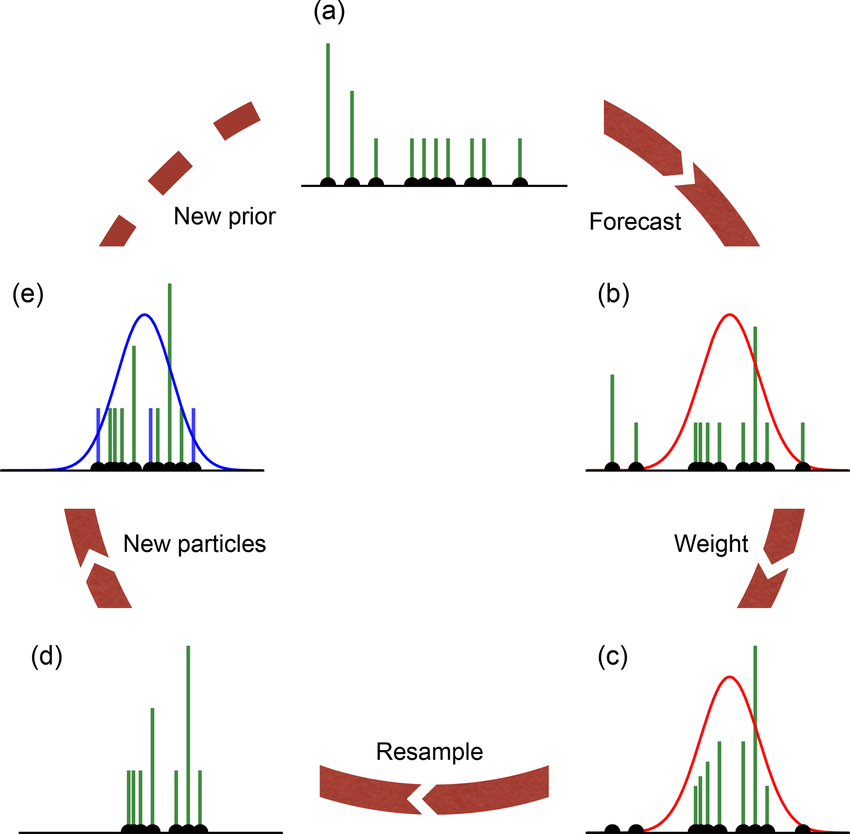
\includegraphics[scale=0.125]{imgs/pfilter.png}
            \end{minipage}
        \begin{minipage}[c]{0.45\textwidth}
            \caption{
            \\
            -- Dirac measure approximation of the Bayes filter. 
            \\ 
            -- Yields a filtering distribution and likelihood estimate.
            \\ 
            -- Graphic from \cite{berg2019pfilterimage}.}
        \end{minipage}
        \label{fig:pfilter-illustration}
    \end{figure}
    
    \begin{itemize}
        \item Monte Carlo approximation of the Bayes filter.
        \begin{itemize}
            \item \pause Maintain $J$ weighted particles, weighted Dirac approximation of the current state $(x_{n,j}^F)_{j=1}^J$. 
            \item \pause Simulate each of the $J$ particles forward to get $x_{n+1,j}^P \sim f_{X_{n+1}|X_n}(\cdot | x_{n,j}^F; \theta)$.
            \item \pause Observe observation $y_{n+1}^*$, update $(x_{n+1,j}^F)_{j=1}^J$ by resampling according to their likelihoods.
        \end{itemize}
    \end{itemize}
\end{frame}

\begin{frame}{Likelihood Estimate}
    \begin{block}{Conditional Likelihood}
        The conditional likelihood $L_n$ under $\theta$ is given by $f_{Y_n|Y_{1:n}}(y_{n}^*|y_{1:n-1};\theta)$.
    \end{block}
    \pause
    \begin{block}{Likelihood}
        \begin{align*}
            \mathcal{L}(\theta)&=f_{Y_{1: N}}\left(y_{1: N}^* ; \theta\right)
            = \prod_{n=1}^N L_n(\theta)\\
            &=\prod_{n=1}^N \int f_{Y_n \mid X_n}\left(y_n^* \mid x_n ; \theta\right) f_{X_n \mid Y_{1: n-1}}\left(x_n \mid y_{1: n-1}^* ; \theta\right) d x_n.
        \end{align*}
    \pause
    An unbiased estimate of the likelihood from the particle filter is then
        $$\hat\lik(\theta) = \prod_{n=1}^N \frac{1}{J}\sum_{j=1}^J f_{Y_n|X_n}(y_n^*|x_{n,j}^P;\theta).$$
    \end{block}
\end{frame}


\begin{frame}{Automatic Differentiation}

    \begin{figure}
        \begin{minipage}[c]{0.7\textwidth}
            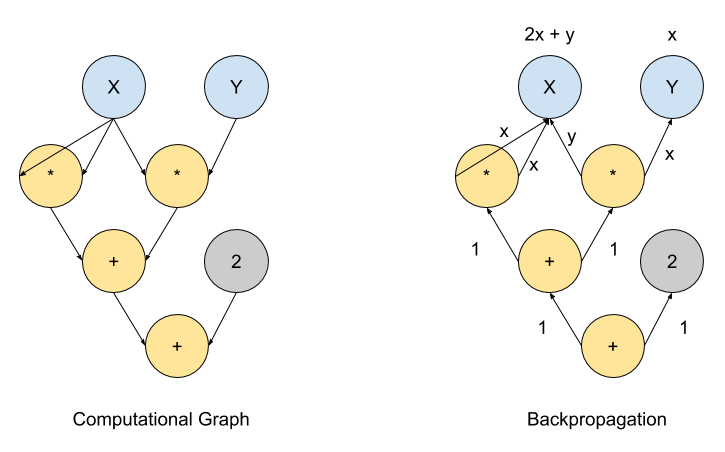
\includegraphics[scale=0.3]{imgs/autograd.png}
        \end{minipage}
        \begin{minipage}[l]{0.27\textwidth}
            \caption{
            \\$f(x,y) = x^2+xy+2$, $f'(x,y) = (2x+y,x).$
            -- Figure from \href{https://avinashselvam.medium.com/automatic-differentiation-explained-9f02c74e9a90}{Medium}.}
        \end{minipage}
        \label{fig:autograd-illustration}
    \end{figure}
    
    \begin{itemize}
        \item Evaluates the gradient of a (scalar or vector-valued) computer program w.r.t. its arguments.
        \item \pause Traverses computational graph (of primitive functions) with chain rule.
    \end{itemize}
    
\end{frame}

\begin{frame}{Maximum Likelihood for POMPs}
    \begin{block}{Iterated Filtering}
        \begin{itemize}
            \item Augment the state space by assigning each particle $x_{n,j}$ its own set of parameters $\theta_{n,j}$. \pause
            \item Parameters thought of as latent states that evolve according to Brownian motion on $\Theta$.  \pause
            \item Yields a Monte Carlo approximation to the (extended) filtering distribution $f_{\theta_n,X_n|Y_{1:n}}(\theta_{n,j},x_{n,j}^F|y_{1:n}^*)$, given a Gaussian random walk prior on $\theta_{n,j} \sim \gN(\theta_{n-1,j},\sigma^2)$. \pause
            \item Repeat procedure again and again, while shrinking $\sigma^2$.\pause
            \item Yields convergence of the parameter swarm $\theta_{n,j}^{(m)}$ to the MLE. 
        \end{itemize}
    \end{block}
\end{frame}


\section{Motivation}

\begin{frame}{Maximum Likelihood Inference is Hard in POMPs}
    
\begin{enumerate}
    \item \textbf{Intractable likelihood functions}! Bypassed with e.g. simulated likelihood, likelihood-free inference, particle filters, etc. 
    \item \pause May not have access to transition densities, only a \textbf{simulator}. 
    \begin{itemize}
        \item \pause IF2 (\cite{ionides15}), particle MCMC (\cite{doucet2010pmcmc}), only full-information methods that can deal with this.
    \end{itemize}
    \item \pause \textbf{Significant Monte-Carlo noise in likelihood estimate} makes accurate parameter estimation difficult.
\end{enumerate}
\end{frame}

\begin{frame}{IF2 Plateaus Quickly But Struggles to Find the MLE}
\begin{figure}
    \centering
    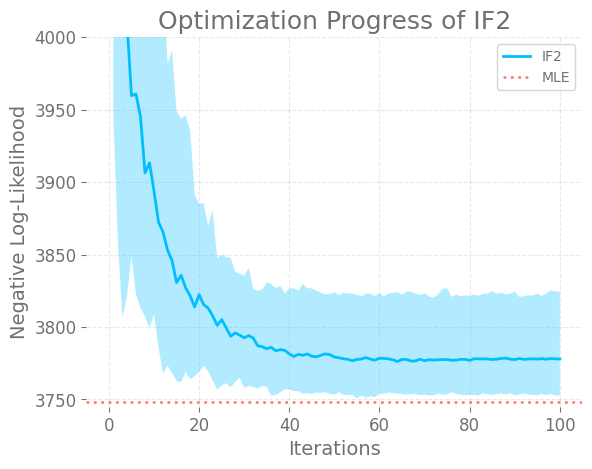
\includegraphics[scale=0.5]{imgs/095/if2fail.png}
    \caption{Performance of IF2 on \cite{king08} Dhaka cholera model. Shaded area represents 0th to 80th percentile, solid line is median of 100 runs. While IF2 makes quick initial progress, it fails to find the MLE.}
    \label{fig:if2fail}
\end{figure}
\end{frame}

\begin{frame}{Hang on, wait a minute!}
    \begin{itemize}
        \item Original iterated filtering algorithm: (noisy) approximation of score (\cite{ionides06-pnas}). 
        %\item \pause Performed a single "gradient step" at the end of each filtering iteration.
        \pause
        \item \textbf{Would performing automatic differentiation (AD) on the likelihood estimate from the particle filter lead to a less noisy score approximation?}
    \end{itemize}
    \pause
    \begin{block}{Problem!}
        But the particle filter has discrete stochastic resampling! How can we differentiate this?
    \end{block}
\end{frame}

\section{Previous Work: AD for Particle Filters}


\begin{frame}{Previous Work}

    \begin{table}[h!]
        \centering
        \begin{tabular}{||c c||} 
         \hline
         Authors & Method \\ [0.5ex] 
         \hline\hline
         \cite{poyiadjis11} & Particle approximation of score.
         \\ & $O(N^2)$ variance, consistent. \\
         \hline
         \cite{blei2018vsmc} & Backprop through vanilla PF. \\ 
         & Asymptotic bias. \\
         \hline
         \cite{corenflos21} & Optimal transport resampling. \\
         & Consistent, $O(J^2)$ runtime. \\
         \hline
         \cite{scibior21} & Stop-gradient trick. \\ 
         & Recovers \cite{poyiadjis11} with AD. \\
         \hline 
         \cite{singh22} & Fixed-lag smoothing. \\ 
         & Need transition densities. \\ 
         \hline
        \end{tabular}
        \label{table:lit-review}
    \end{table}
\end{frame}


\begin{frame}{Our Contributions}
    \begin{itemize}
        \item New theoretical framework/algorithm/gradient estimator we call MOP-$\alpha$.
        \begin{itemize}
            \item \pause Gradient estimates of \cite{blei2018vsmc} (MOP-0), \cite{poyiadjis11} and \cite{scibior2021dpf} (MOP-1) are special cases.
            \item \pause Does not need transition densities, only a differentiable simulator.
            \item \pause Can optimize a bias-variance tradeoff. 
        \end{itemize}
        \item \pause Promising hybrid algorithm, warm-starts gradient descent (using this estimator) with IF2.
        \item \pause Outperforms IF2 on Cholera model of \cite{king08}.
    \end{itemize}
\end{frame}


\section{Smooth Extensions to the Particle Filter}

\begin{frame}{Intuition}
    \begin{block}{Problem}
        Want to differentiate through the particle filter. But the particle filter has discrete stochastic resampling! 
    \end{block}
    \pause 
    \begin{block}{Idea}
        Don't differentiate $\hat\ell(\theta)$ directly, differentiate through a simulator and a series of measurement density ratios.
    \end{block}
    \begin{itemize}
        \item \pause Particle filter run with state transitions \& resampling under $\phi \in \Theta$. 
        \item \pause Get a coupled (same seed) set of particles according to the process model at $\theta \in \Theta$, but resampling indices from the run at $\phi$. 
        \item \pause Reweight conditional likelihoods by a correction factor accumulated over time, to account for resampling under $\phi$. 
        \item \pause If $\theta=\phi$, need only one run, else need two runs at same seed. 
    \end{itemize}
\end{frame}

\begin{frame}{What is the correction?}
    \begin{block}{Correction}
        \begin{itemize}
            \item Write:\pause
            \begin{itemize}
                \item $g^{\theta}_{n,j}={f}_{{Y}_{n}|{X}_{n}}(y_{n}^{*}|{X}_{n,j}^{P,\theta}\giventh{\theta})$ for the measurement density.\pause
                \item $L_n^{\phi} = \frac{1}{J}\sum_{m=1}^{J}g^{\phi}_{n,m}$ for the conditional likelihood estimate under $\phi$.\pause
                \item $k_j \sim \text{Categorical}(g^{\phi}_{n,1},...,g^{\phi}_{n,J})$ for the resampling indices under $\phi$. \pause
            \end{itemize}
            \item Estimate conditional likelihood under $\theta$ as
            \pause
            \begin{equation}
     \label{eq:mop-conditional-likelihood}
     \underbrace{L_n^{B,\theta,\alpha} = \frac{\sum_{j=1}^Jg^\theta_{n,j} w^{P,\theta}_{n,j}}{\sum_{j=1}^J  w^{P,\theta}_{n,j}}}_{\textcolor{blue}{\text{\tiny{Usual way to estimate functionals under particle filter.}}}} \text{ or } \underbrace{L_n^{A,\theta,\alpha} = L_n^\phi\cdot \frac{\sum_{j=1}^J w^{F,\theta}_{n,j}}{\sum_{j=1}^J  w^{P,\theta}_{n,j}}}_{\textcolor{red}{\text{\tiny{Higher variance, but useful for derivations.}}}},
    \end{equation}
    \pause
    recursively weighting each particle by 
    \pause
    \begin{equation}
        \label{eq:weighting-scheme}
        \underbrace{w_{n,j}^{P,\theta} = (w_{n-1,j}^{F,\theta})^\alpha}_{\textcolor{red}{\text{\tiny{Bias-variance tradeoff.}}}}, \;\; \underbrace{w^{F,\theta}_{n,j} = w^{P,\theta}_{n,k_j} { g^{\theta}_{n,k_j}}/{ g^{\phi}_{n,k_j}}}_{\textcolor{blue}{\text{\tiny{Resampling correction.}}}}, \;\; w^{F,\theta}_{0,j}= 1.
    \end{equation}
        \end{itemize}
    \end{block}
\end{frame}


\begin{frame}{Algorithm: Measurement Off-Policy, MOP-$\alpha$}
    \begin{enumerate}
        \item \textbf{Run a particle filter once at} $\phi$ to obtain $X_{n,j}^{P,\phi}, X_{n,j}^{F,\phi}$. Fix seed throughout. Set initial weights $w_{0,j}^{F,\theta} = 1/J$.
        \item \pause \textbf{At each timestep,} propagate weights $w_{n,j}^{P,\theta} := (w_{n-1,j}^{F,\theta})^\alpha$. 
        \item \pause Simulate process model ${X}_{n,j}^{P,\theta}\sim {f}_{{X}_{n}|{X}_{n-1}}\big(\cdot|{X}_{n-1,j}^{F};{\theta}\big)$, evaluate measurement model $g^{\theta}_{n,j}={f}_{{Y}_{n}|{X}_{n}}(y_{n}^{*}|{X}_{n,j}^{P,\theta}\giventh{\theta})$, evaluate conditional likelihood under $\phi$, $L_n^{\phi} = \frac{1}{J}\sum_{m=1}^{J}g^{\phi}_{n,m}$, \textbf{as usual.}
        \item \pause \textbf{Resample according to $\phi$:} $k_{1:J} \sim \prob\big(k_{j}=m\big) \propto g^{\phi}_{n,m}$.
        \item \pause \textbf{Correct filtering weights:} $\displaystyle w^{F,\theta}_{n,j}= w^{P,\theta}_{n,k_j} \times  g^{\theta}_{n,k_j}/ g^{\phi}_{n,k_j}$. 
    \end{enumerate}
    \pause 
    \centering{\textbf{Special Case:} If $\theta=\phi$, only need to run one particle filter! Set $X_{n,j}^{P,\theta}, X_{n,j}^{F,\theta}$ to be copies of the $\phi$ counterparts, where gradients don't propagate. Explains the \textbf{stop-gradient} trick of \cite{scibior21}.}
\end{frame}


\begin{frame}{Bias-Variance Tradeoff with $\alpha$}
\begin{itemize}
    \item $\alpha$ balances a tradeoff between:
    \begin{itemize}
        \item \pause Maintaining memory of each particle's ancestral trajectory (most extreme when $\alpha=1$).
        \item \pause High-variance, but consistent.
        \item \pause Considering only the single-step transition dynamics (when $\alpha=0$).
        \item \pause Low-variance, but asymptotically biased.
    \end{itemize}
    \item \pause\textbf{Exponentially-weighted moving average} where $\alpha$ controls the amount of discounting.
    \item \pause Bias small if $y_{n+1:N}^*$ not informative for $x_n$ given $y_{0:n}^*$ (\cite{corenflos21}).
\end{itemize}
    
\end{frame}


\begin{frame}{Bias-Variance Tradeoff with $\alpha$}
\begin{figure}
    \centering
    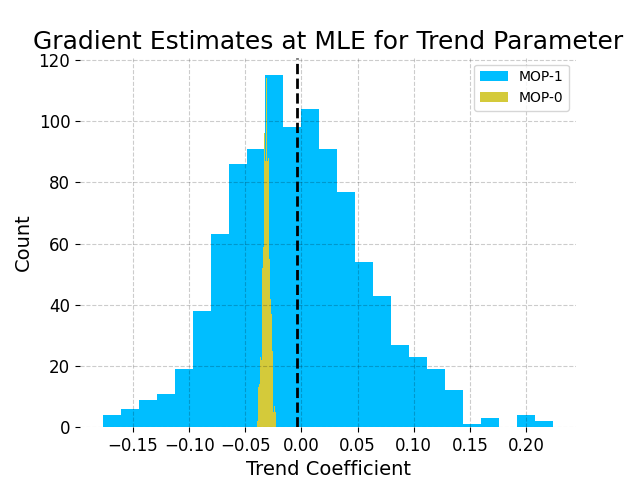
\includegraphics[scale=0.5]{imgs/mlegrad.png}
    \caption{Gradient estimates at MLE for trend in \cite{king08} cholera model. When $\alpha=1$, estimate close to unbiased with high variance. When $\alpha=0$, lower variance but biased.}
    \label{fig:bias-variance}
\end{figure}
    
\end{frame}


\begin{frame}{Bias-Variance Tradeoff with $\alpha$}
\begin{figure}
    \centering
    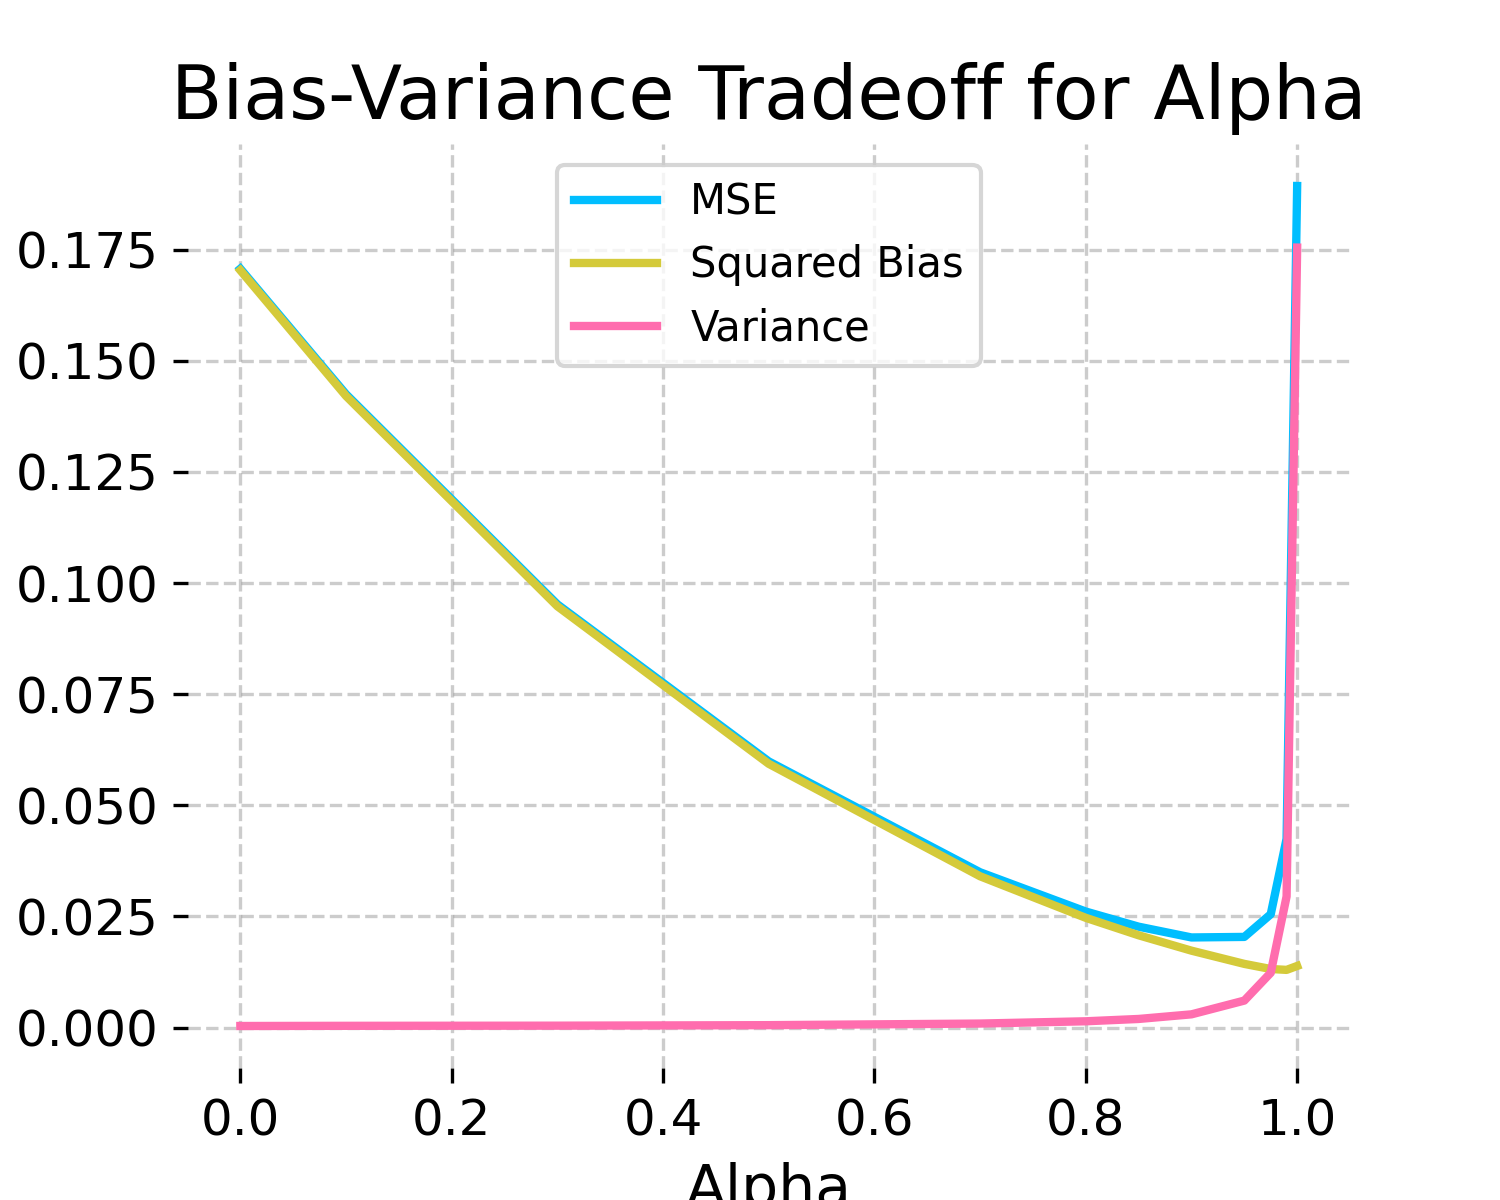
\includegraphics[scale=0.5]{imgs/095/biasvar.png}
    \caption{Bias-variance tradeoff for gradient estimates at MLE for trend in \cite{king08} cholera model. When $\alpha=1$, estimate close to unbiased with high variance. When $\alpha=0$, lower variance but biased. MSE minimized at $\alpha=0.97$.}
    \label{fig:bias-variance}
\end{figure}
    
\end{frame}


\section{Theoretical Guarantees}

\begin{frame}{Assumptions}
    
\begin{itemize}
    \item \textbf{Continuity of the Likelihood.} $\ell(\theta)$ has more than two continuous derivatives in a neighborhood of the MLE.
    \pause
    \item \textbf{Bounded Process Model.} There exist $\underbar{M}, \bar{M}$ bounding the process density from below/above.
    \pause
    \item \textbf{Bounded Measurement Model.} $\underbar{G}, \bar{G}$ bound the measurement density from below/above, and $G'(\theta)<\infty$ bounding its gradients.
    \pause
    \item \textbf{Bounded Gradient Estimates.} There are functions $G(\theta), H(\theta): \Theta \to [0,\infty)$ so the MOP-$\alpha$ gradient and Hessian estimates at $\theta=\phi$ are bounded by $G(\theta)$ and $H(\theta)$.
    \pause
    \item \textbf{Differentiability of Density Ratios and Simulator.} The measurement density $f_{Y_n|X_n}(y_n^*|x; \theta)$ and simulator have more than two continuous derivatives in $\theta$.
\end{itemize}
\end{frame}

\begin{frame}{MOP-$\alpha$ Works}
    \begin{thm}[MOP-$\alpha$ Targets the Posterior and Likelihood]
    \label{thm:mop-targeting}
    When $\alpha=1$ or $\theta=\phi$, MOP-$\alpha$ targets the posterior and is strongly consistent for the likelihood, as the number of particles $J \to \infty$.
    
    \pause
    That is, for $\pi_n(\theta)=f_{X_{1:n}|Y_{1:n} ; \theta}$ and any measurable bounded functional $h$, 
    \pause
    \begin{equation}
        \underbrace{\frac{\sum_{j=1}^J h(x_{n,j}^{A,F, \theta}) w_{n,j}^{A,F,\theta}}{\sum_{j=1}^J w_{n,j}^{A,F,\theta}} \stackrel{a.s.}{\to} E_{\pi_n(\theta)} h,}_{\textcolor{blue}{\text{\tiny{Particle estimates of functionals under the posterior are consistent.}}}} \;\; \underbrace{\hat\lik(\theta)  \stackrel{a.s.}{\to} \lik(\theta).}_{\textcolor{red}{\text{\tiny{Likelihood estimate is consistent.}}}}
    \end{equation}
\end{thm}
\end{frame}

\begin{frame}{Proof Sketch}
    \begin{itemize}
        \item This also serves as a strong law of large numbers result for triangular arrays of particles with ``off-policy'' resampling.\pause
        \item When $\theta=\phi$, the ratio ${g_{n,j}^\theta}/{g_{n,j}^\phi}=1,$ and this reduces to the vanilla particle filter! Everything is as per usual. \pause
        \item  When $\alpha=1$ and $\theta\neq\phi,$ suppose inductively that $\{(X^{F,\theta}_{n-1,j},w^{F,\theta}_{n-1,j})\}_{j=1}^J$ targets $f_{X_{n-1}|Y_{1:n-1}}(x_{n-1}|y^*_{1:n-1};\theta)$.\pause 
        \begin{itemize}
            \item We show $\{(X^{P,\theta}_{n,j},w^{P,\theta}_{n,j})\}_{j=1}^J$ targets $f_{X_{n}|Y_{1:n-1}}(x_{n}|y^*_{1:n-1};\theta)$.\pause
            \item $\{(X^{P,\theta}_{n,j},w^{P,\theta}_{n,j} g^\theta_{n,j} )\}_{j=1}^J$ targets  $f_{X_{n}|Y_{1:n}}(x_{n}|y^*_{1:n};\theta)$. \pause
            \item And that weighting by $(X^{F,\theta}_{n,j},w^{F,\theta}_{n,j}) = (X^{P,\theta}_{n,a(j)}, w^{P,\theta}_{n,a(j)} g^\theta_{n,a(j)}/ g^\phi_{n,a(j)})$ and resampling with probabilities $g^\phi_{n,j}$, targets $f_{X_{n}|Y_{1:n}}(x_{n}|y^*_{1:n};\theta)$.\pause
        \end{itemize}
        \item Result relies on three lemmas that are ``common-sense'' but require somewhat technical arguments to prove. 
    \end{itemize}
\end{frame}

\begin{frame}{MOP-$\alpha$ Special Cases}
    \begin{thm}[MOP-$0$ and MOP-$1$ Functional Forms]
    \label{thm:mop-functional-forms}
    Write $\nabla_\theta \hat\ell^\alpha(\theta)$ for the gradient estimate yielded by MOP-$\alpha$ when $\theta=\phi$ and we use the after-resampling conditional likelihood estimate. When $\alpha=0$,
    \pause
    \begin{equation}
        \nabla_\theta \hat\ell^0(\theta) 
        = \frac{1}{J} \sum_{n=1}^N \sum_{j=1}^J \nabla_\theta \log\left(f_{Y_n|X_{n}}(y_n^*|x_{n,j}^{F, \theta}; \theta)\right),
        \vspace*{-2.5mm}
    \end{equation}
    \pause
    yielding \cite{blei2018vsmc} on the bootstrap filter. When $\alpha=1$,
    \pause
    \begin{equation}
        \nabla_\theta \hat{\ell}^1(\theta) 
        = \frac{1}{J}\sum_{j=1}^J \nabla_\theta \log f_{Y_{1:N}|X_{1:N}}\left(y_{1:N}^* | x_{1:n,j}^{A, F,\theta}\right),
    \vspace*{-2.5mm}
    \end{equation}
    \pause
    yielding the estimator of \cite{poyiadjis11} with the bootstrap filter.
\end{thm}
\pause
Proof: Very tedious algebra.
\end{frame}

\begin{frame}{MOP-$1$ Is Strongly Consistent for the Score}
    \begin{itemize}
        \item But \cite{poyiadjis11} use $\frac{1}{J}\sum_{j=1}^J \nabla_\theta \log f_{Y_{1:N}, X_{1:N}}\left(y_{1:N}^* , x_{1:n,j}^{A, F,\theta}; \theta\right)$ in general. \pause
        \item The bootstrap estimate of $\nabla_\theta \hat{\ell}^1(\theta) 
        = \frac{1}{J}\sum_{j=1}^J \nabla_\theta \log f_{Y_{1:N}|X_{1:N}}\left(y_{1:N}^* | x_{1:n,j}^{A, F,\theta}\right)$ has a different functional forms, and is not the same a-priori! \pause
        \item So we directly show the consistency of the MOP-$1$ gradient estimate. 
    \end{itemize}
    \pause
    \begin{thm}[Consistency of MOP-$1$ Gradient Estimate]
        The gradient estimate of MOP-$\alpha$ when $\alpha=1$, $\theta=\phi$ is strongly consistent for the score: $\nabla_\theta \hat\ell_J^1(\theta) \stackrel{a.s.}{\to} \nabla_\theta \ell(\theta)$ as $J \to \infty$.
        \label{thm:mop-grad-consistency}
    \end{thm}
\end{frame}

\begin{frame}{Proof of MOP-$1$ Gradient Estimate Consistency}
    \begin{itemize}
        \item The sequence $(\hat\lik_J^1(\theta)(\omega))_{J \in \mathbb{N}}$ has two derivatives uniformly bounded over all $J$, by assumption. \pause
        \item So $(\nabla_\theta \hat\lik_J^1(\theta)( \omega))_{J \in \mathbb{N}}$ is uniformly Lipschitz, and therefore uniformly equicontinuous for almost every $\omega \in \Omega$.\pause
        \item By Arzela-Ascoli, there is a uniformly convergent subsequence. \pause
        \item But there is only one subsequential limit by Theorem \ref{thm:mop-targeting}!\pause
        \item So the whole sequence must converge uniformly with $\hat{\lik}_J^1(\theta, \omega) \stackrel{a.s.}{\to} \lik(\theta)$. \pause
        \item So we can swap the limit and derivative and obtain that for almost every $\omega \in \Omega$, 
    $\lim_{J \to \infty} \nabla_\theta \hat\lik_J^1(\theta)(\omega) = \nabla_\theta \lim_{J \to \infty} \hat\lik_J^1(\theta)(\omega) = \nabla_\theta \lik(\theta).$\pause
        \item The result then follows by the continuous mapping theorem. 
    \end{itemize}
\end{frame}

\begin{frame}{MOP-$\alpha$ Variance Bound}
    \begin{thm}[MOP-$\alpha$ Variance Reduction]
        The variance of the MOP-$\alpha$ gradient estimate, for $\alpha<1$, is given by
        \pause
        $$\text{Var}(\nabla_\theta \hat\ell^\alpha(\theta)) \lesssim \min_{k\leq N} \left(\underbrace{\frac{k^2G'(\theta)^2N}{(1-\alpha)^2J}}_{\textcolor{blue}{\tilde O(Nk^2/J)}} + \underbrace{\frac{16\alpha^{2k}}{(1-\alpha)^2}N^2G'(\theta)^2}_{\textcolor{red}{\text{\tiny{Decreasing exponentially in $k$.}}}} \right).$$
    \end{thm}
    \pause
    \begin{itemize}
        \item Low-variance MOP-$0$ from \cite{blei2018vsmc} has $\tilde{O}(N/J)$ variance (we show this).\pause
        \item High-variance MOP-$1$ from \cite{poyiadjis11} has $\tilde{O}(N^4/J)$ variance. \pause
        \item MOP-$\alpha$ interpolates through both of these results to balance a bias-variance tradeoff. 
    \end{itemize}
\end{frame}

\begin{frame}{Proof Sketch of MOP-$\alpha$ Variance Bound}
    \begin{itemize}
        \item Long and ugly.\pause
        \item Consider a ``truncated'' version of the MOP-$\alpha$ estimate, where the weight correction is truncated at $k$ timesteps. This is easier to analyze. \pause
        \item Call the conditional log-likelihood estimate $\hat{s}_{n,k}$, log-likelihood estimate $\hat{s}_{k}$, score estimate $\nabla_\theta \hat{s}_{k}$.\pause
        \item By tedious algebra, the deviation of the truncated score estimate from the MOP-$\alpha$ score estimate is $\left\lVert\nabla_\theta\hat\ell(\theta) - \hat s_k(\theta) \right\rVert_\infty \leq  \frac{2\alpha^k}{1-\alpha}NG'(\theta)$.\pause
        \item Single-timestep variance is bounded by $\E\left[||\hat s_{n,k}(\theta) - \E_{\pi}\hat s_{n,k}(\theta)||_\infty^2\right]^{1/2} \leq \frac{Cr^2G'(\theta) k}{\sqrt{J}}.$
    \end{itemize}
\end{frame}

\begin{frame}{Proof Sketch, Continued}
\begin{align*}
    \text{Var}(\nabla_\theta \hat s_k(\theta)) 
    &= \sum_{n=1}^N\text{Var}\left(\hat s_{n,k}(\theta)\right)+ 2\sum_{m<n}\text{Cov}\left(\hat s_{m,k}(\theta), \hat s_{n,k}(\theta)\right) \\
    &\lesssim \frac{r^2k^2G'(\theta)^2N}{J} + 2\sum_{m<n}\text{Cov}\left(\hat s_{m,k}(\theta), \hat s_{n,k}(\theta)\right).
\end{align*}
\pause
    \begin{itemize}
        \item How do we control the covariance? Mixing argument!\pause
        \item Mixing time of the particle filter is $O(\log(J))$, \cite{karjalainen2023}. \pause
        \item $\hat s_{n,k}$ is strong mixing at lag $k+1$, as weights beyond $k$ timesteps are truncated. \pause
        \item So the $\alpha$-mixing coefficients for $(\hat s_{n,k}(\theta))_{n=1}^N$ are given by $\alpha(l) \leq (1-\epsilon)^{\floor{l/(c(1+k+\log(J)))}}$. 
    \end{itemize}
\end{frame}

\begin{frame}{Proof Sketch, Continued}
    \begin{itemize}
        \item By Davydov's inequality and Lemma 2 of \cite{karjalainen2023}, we can show that \pause
    $$\text{Cov}\left(\hat s_{m,k}(\theta), \hat s_{n,k}(\theta)\right) \lesssim (1-\epsilon)^{\frac{1}{2}\floor{\frac{|n-m|}{c(1+k+\log(J))}}}\frac{r^2G'(\theta)^2}{J}.$$
    \pause
    \item Recall that $||\nabla_\theta\hat\ell(\theta) - \hat s_k(\theta)||_\infty \leq \frac{2\alpha^k}{1-\alpha}NG'(\theta)$.\pause
    \item So we have that for any $k\leq N$,
    $$\text{Var}(\nabla_\theta \hat\ell(\theta)) \lesssim \frac{k^2r^2G'(\theta)^2N}{J} + \frac{16\alpha^{2k}}{(1-\alpha)^2}N^2G'(\theta)^2.$$
    \pause
    \item Take the minimum over $k$ to get the result. 
    \end{itemize}
\end{frame}

\section{Practical Maximum Likelihood Inference}

\begin{frame}{One possible procedure:}
    \begin{itemize}
        \item Warm-start gradient descent, or some other first or second order procedure (using the gradient estimate given by MOP-$\alpha$), with the output of an initial search of IF2. 
        \item \pause Run IF2, aggressively cooling to a fixed learning rate, till search stalls.
        \item \pause Refine this coarse solution with gradient descent.
    \end{itemize}
    \pause
    \centering{\textbf{Iterated Filtering with Automatic Differentiation (IFAD)}}
\end{frame}


\begin{frame}{Convergence Analysis}
    \begin{prop}[Linear Convergence of IFAD-1]
        \label{thm:convergence}
        
        Consider a variant of IFAD-1 stopping if the gradient estimate $||g(\theta_n)|| \leq \sigma \epsilon$. Assume $-\ell$ is $\gamma$-strongly convex, $\gamma I \preceq \nabla_\theta^2 (-\ell) \preceq \Gamma I$. $\sigma = \frac{4 \Gamma}{(1-\beta)}> 4$.
        
        Let $H(\theta_n)$ be a matrix possibly dependent on $\theta_n$ with minimum eigenvalue always greater than some $c>0$. Choose learning rate $\eta$ and error tolerance $\epsilon$ such that, where $\beta$ is the Armijo condition hyperparameter,
        \begin{equation*}
            \eta \leq \frac{c(1-\beta)}{\Gamma}, \;\; \epsilon \leq \frac{c(1-\beta)}{2\Gamma}||g(\theta_n)||.
        \end{equation*}
        
        Then, with $J$ large enough, the following holds with probability at least $1-\delta$:
        \begin{equation*}
        \ell(\theta^*) - \ell(\theta_{n+1}) \leq \left(1-\eta\beta\frac{8\gamma}{9c}\right)(\ell(\theta^*)-\ell(\theta_n))
        \end{equation*}
        
        and the algorithm terminates when $||\nabla_\theta \ell(\theta_n)|| \leq (1+\sigma) \epsilon$.
        \end{prop}
\end{frame}

\begin{frame}{Convergence Analysis}
    \begin{itemize}
        \item Similar to \cite{mahoney16}, uses concentration inequalities from \cite{delmoral2011ci}.
        \item Gradient stage of IFAD-1 converges linearly to the MLE if:
        \begin{enumerate}
            \item \pause The log-likelihood surface is $\gamma$-strongly convex in a neighborhood of the MLE.
            \item \pause The IF2 stage of IFAD successfully reaches a (high-probability) basin of attraction of the MLE. 
        \end{enumerate}
        \item \pause \textbf{Conjecture:} This applies to the entirety of IFAD, as IF2 converges very quickly to a neighborhood of the MLE and behaves a lot like SGD. 
    \end{itemize}
    
\end{frame}


\begin{frame}{Runtime}

\begin{itemize}
    \item Warm-start:
    \begin{itemize}
        \item \pause Initial warm-start "convergence" happens fairly quickly in practice. 
        \begin{itemize}
            \item \pause Dhaka cholera model of \cite{king08}: 40 iterations, usually 100-200 for global search.
        \end{itemize}
    \end{itemize}
    \item \pause MOP-$\alpha$:
    \begin{itemize}
        \item \pause Gradient takes 3.75x time of \texttt{pfilter()}, in line with cheap gradient principle (\cite{kakade2019provably}).
    \end{itemize}
    \item \pause Runtime \textbf{linear, and not quadratic}, in number of particles.
    \item \pause Re-implementation in \texttt{JAX} (\cite{jax2018github}) led to 16x speedup v.s. \texttt{pomp} package of \cite{king08}.
\end{itemize}

\end{frame}


\section{Numerical Experiments}

\begin{frame}{Cholera in Bangladesh}

    \begin{figure}
        \centering
        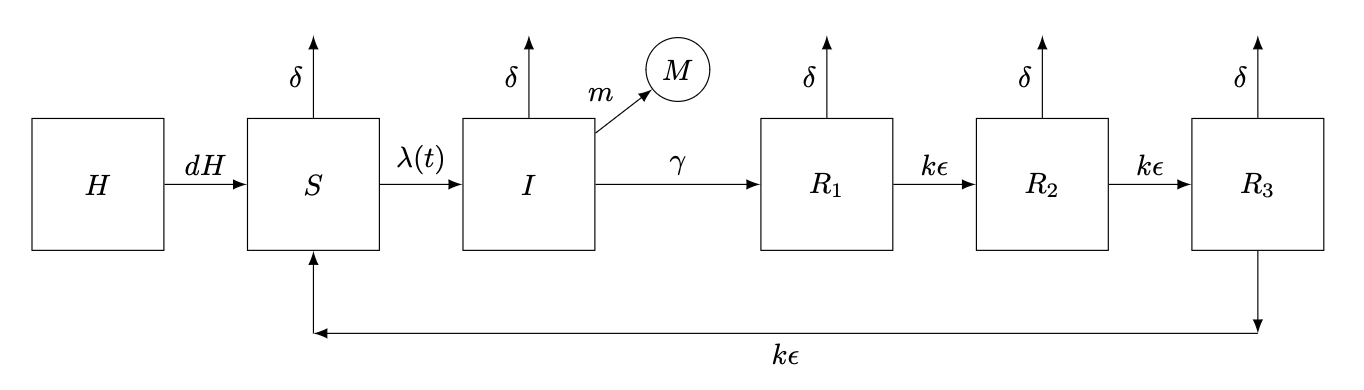
\includegraphics[scale=0.5]{imgs/dacca.png}
        \caption{Illustration of SIR model from \cite{king08}.}
        \label{fig:sir}
    \end{figure}
    
    \begin{itemize}
        \item Dhaka model from \cite{king08}, also used in \cite{ionides15} to benchmark IF2.
        \item \pause Stochastic SIR compartmental model with transition uncertainty driven by Brownian motion.
        \item \pause Force of infection $\lambda(t)$ modeled with splines for seasonality, etc.
    \end{itemize}
    
        %\item \pause Population $H(t)$ divided into:
        %\begin{itemize}
        %    \item \pause Susceptible compartment $S(t)$.
        %    \item \pause Infected compartment $I(t)$.
        %    \item \pause Three ($k=3$) recovered compartments $R_1(t), ..., R_k(t)$ denoting varying degrees of cholera immunity.
        %\end{itemize}
        %\item \pause $M(t)$ denotes the cholera deaths in each month.
\end{frame}

\begin{frame}{Results}
    
    \begin{table}[h!]
        \centering
        \begin{tabular}{||c c c||} 
         \hline
         Method & Best Log-Likelihood & Rank \\ [0.5ex] 
         \hline\hline
         IFAD-0.97 & $\textbf{-3750.21}$ & 1\\
         IFAD-0 & $-3752.17$ & 2\\
         IFAD-1 & $-3754.63$ & 3\\
         IF2 (Ours) & -3764.10 & 4\\
         IF2 (\cite{ionides15}) & -3768.63 & 5\\ 
         MOP-1 Alone (100 searches) & -3797.38 & 6\\
         \hline

        \end{tabular}
        \caption{\\
        -- IFAD performs the best among all methods, finding the MLE. \\
        -- Our implementation of IF2 outperforms that of \cite{ionides15} but underperforms IFAD.}
        \label{table:mle}
    \end{table}
    
    \begin{itemize}
        \item Benchmarked IFAD against IF2 on a challenging global search problem. 
        \item \pause Performed 44 searches each. 
    \end{itemize}
    
\end{frame}

\begin{frame}{Results}
    
\begin{figure}[htbp!]
    \centering
    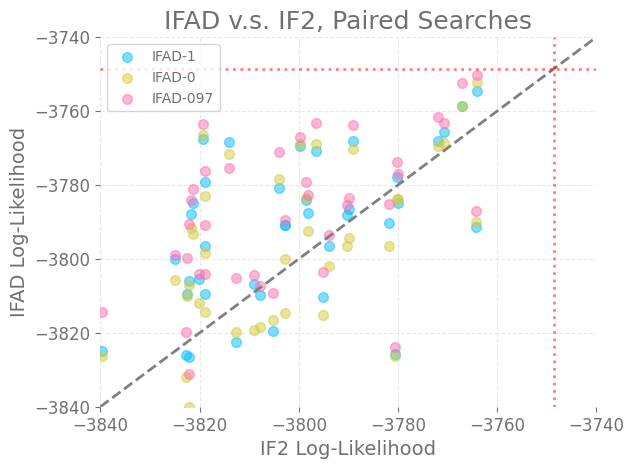
\includegraphics[scale=0.37]{imgs/095/pairs.png}
    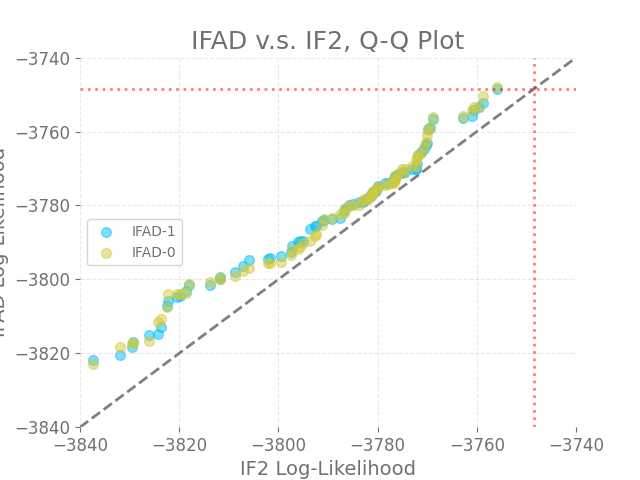
\includegraphics[scale=0.37]{imgs/095/qq.png}
    \caption{\\
    --\textbf{Left:} Paired searches from the same starting point. \\
    --\textbf{Right:} Q-Q plot of ranked IFAD searches against ranked IF2 searches. \\
    -- IFAD has the edge and manages to find the MLE.\\
    -- No IF2 search successfully gets within 7 log-likelihood units of it.}
    \label{fig:scatter}
\end{figure}
\end{frame}

\begin{frame}{Results}
    
\begin{figure}[H]
    \centering
    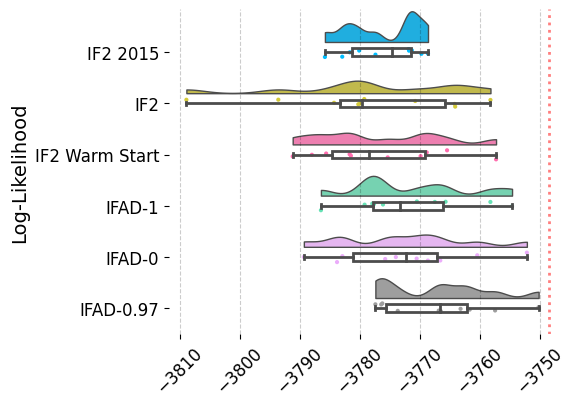
\includegraphics[scale=0.5]{imgs/095/boxplot.png}
    \caption{Results of best run out of every ten runs, simulating procedure of running a few searches and choosing the best one. IFAD outperforms IF2, and tuning $\alpha$ ultimately helps a lot.}
    \label{fig:boxplot-search}
\end{figure}

\end{frame}

\begin{frame}{Results}
\begin{figure}[htbp!]
    \centering
    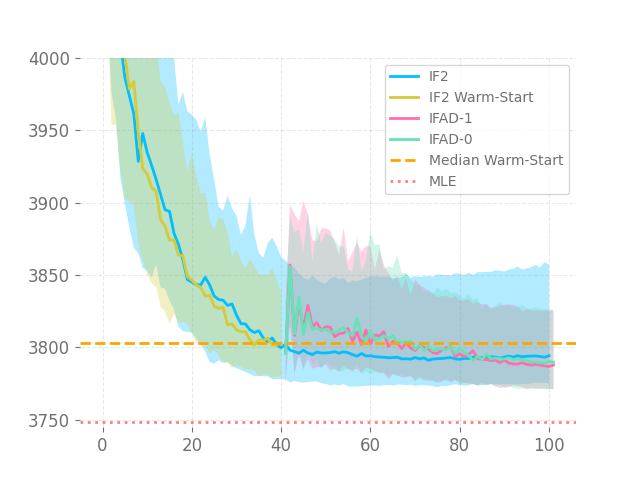
\includegraphics[scale=0.5]{imgs/095/optim.png}
    \caption{\\
    -- Solid lines depict the median negative log-likelihood at each iteration.\\
    -- Shaded area depicts the best search at any iteration and the 80\% percentile.}
    \label{fig:optim}
\end{figure}
%-- While running 60 more iterations of IF2 improves upon the median warm-start, doing so ultimately underperforms IFAD -- IFAD has better tail control and successfully reaches the MLE. The initial loss in log-likelihood upon transitioning from IF2 to MOP seems to help with escaping local minima. 
\end{frame}

\begin{frame}{Results}
    
\begin{figure}[u!]
    \centering
    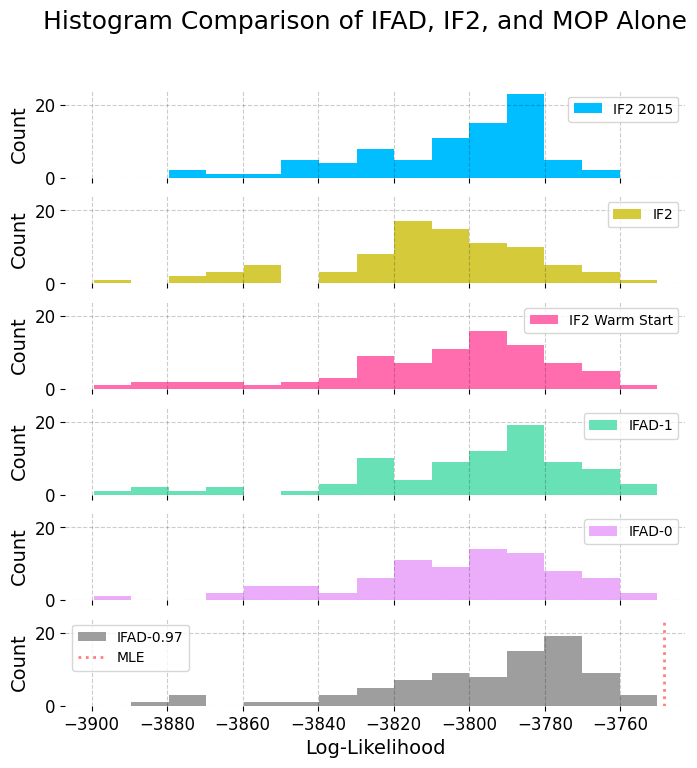
\includegraphics[scale=0.35]{imgs/095/hist.png}
    \caption{Histogram comparison of IFAD, IF2, and MOP alone. Right is better.}
    \label{fig:hist-all}
\end{figure}
\end{frame}

\begin{frame}{Takeaways}
    \begin{enumerate}
        \item IF2 converges quickly to a neighborhood of the MLE but fails to find the MLE.
        \item \pause Gradient steps perform better at fine-grained refinement.
        \item \pause Performing gradient steps alone without a warm-start leads to the search getting stuck in local minima and saddle points.
        \item \pause IFAD combines the best of IF2 and MOP, approaching the MLE quickly and successfully performing refinement -- even on a very difficult global search problem.
    \end{enumerate}
\end{frame}

\section{Extension to Bayesian Inference}

\begin{frame}{Particle MCMC}
    One can use the likelihood estimate from the particle filter to perform MCMC. But the random walk proposal is very bad!
    
\begin{figure}[t!]
    \centering
    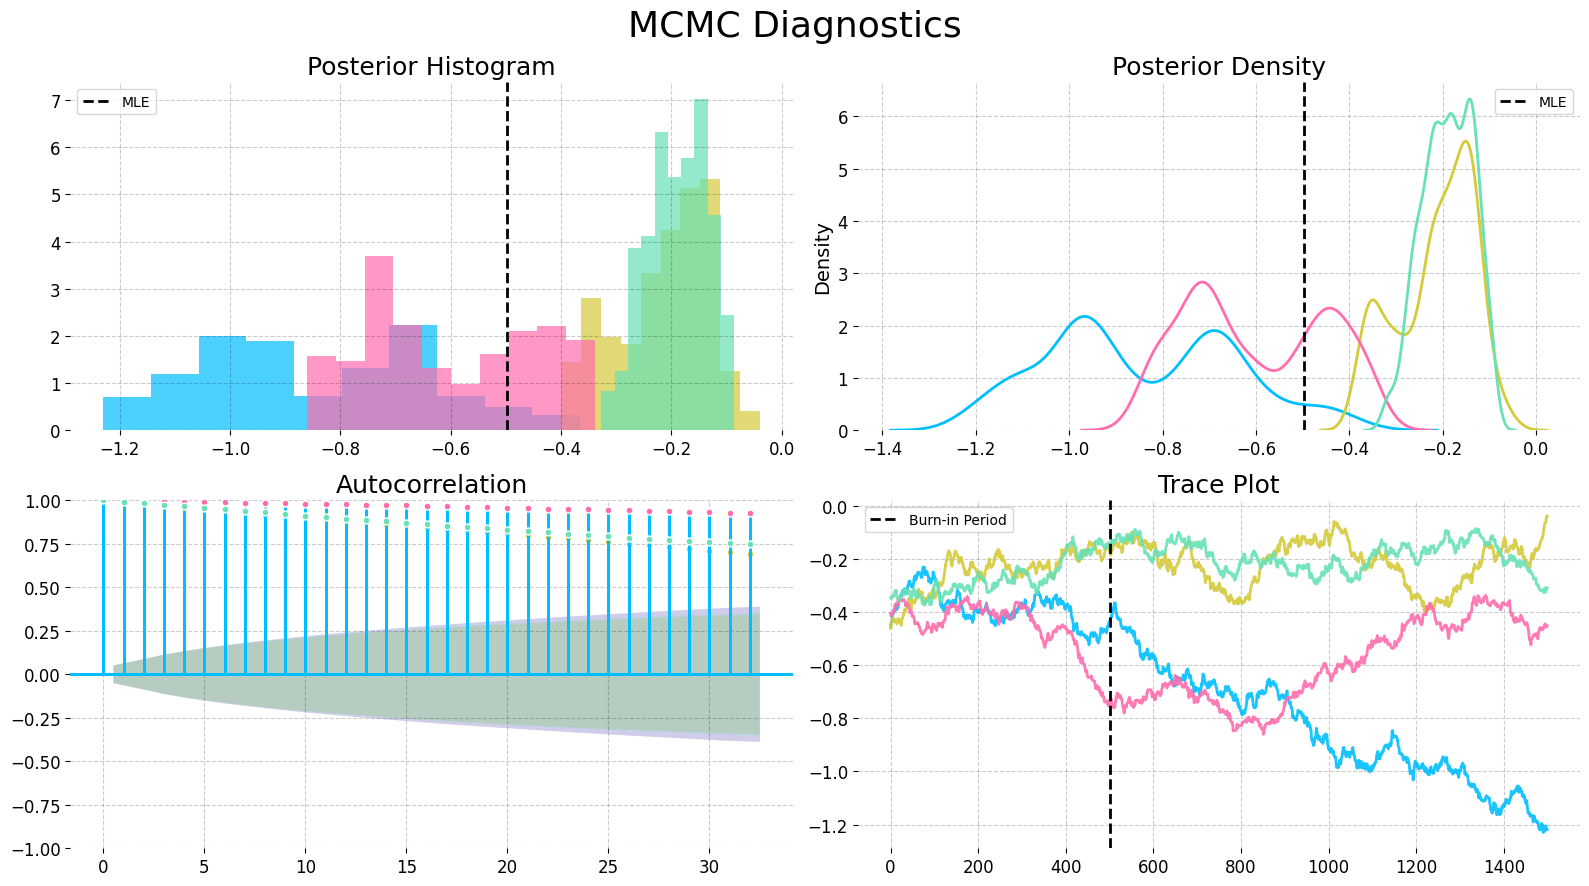
\includegraphics[width = \textwidth/\real{1.5}]{imgs/pmcmc/mh.png}
    \caption{Convergence diagnostics for the Metropolis-Hastings variant particle MCMC with the random walk proposal and an informative empirical prior from IF2. Here, we display the results for the trend parameter in the Dhaka cholera model of \cite{king08}.}
    \label{fig:mh}
\end{figure}
\end{frame}

\begin{frame}{MOP-$\alpha$ Speeds up the Mixing of Particle MCMC}
    Using the gradient estimate from MOP-$\alpha$ within a NUTS sampler (initialized with an informative prior estimated with IF2) works wonders -- burn-in period of $700,000$ in \cite{fasiolo16} reduced to $500$ here.
    \begin{figure}[t!]
    \centering
    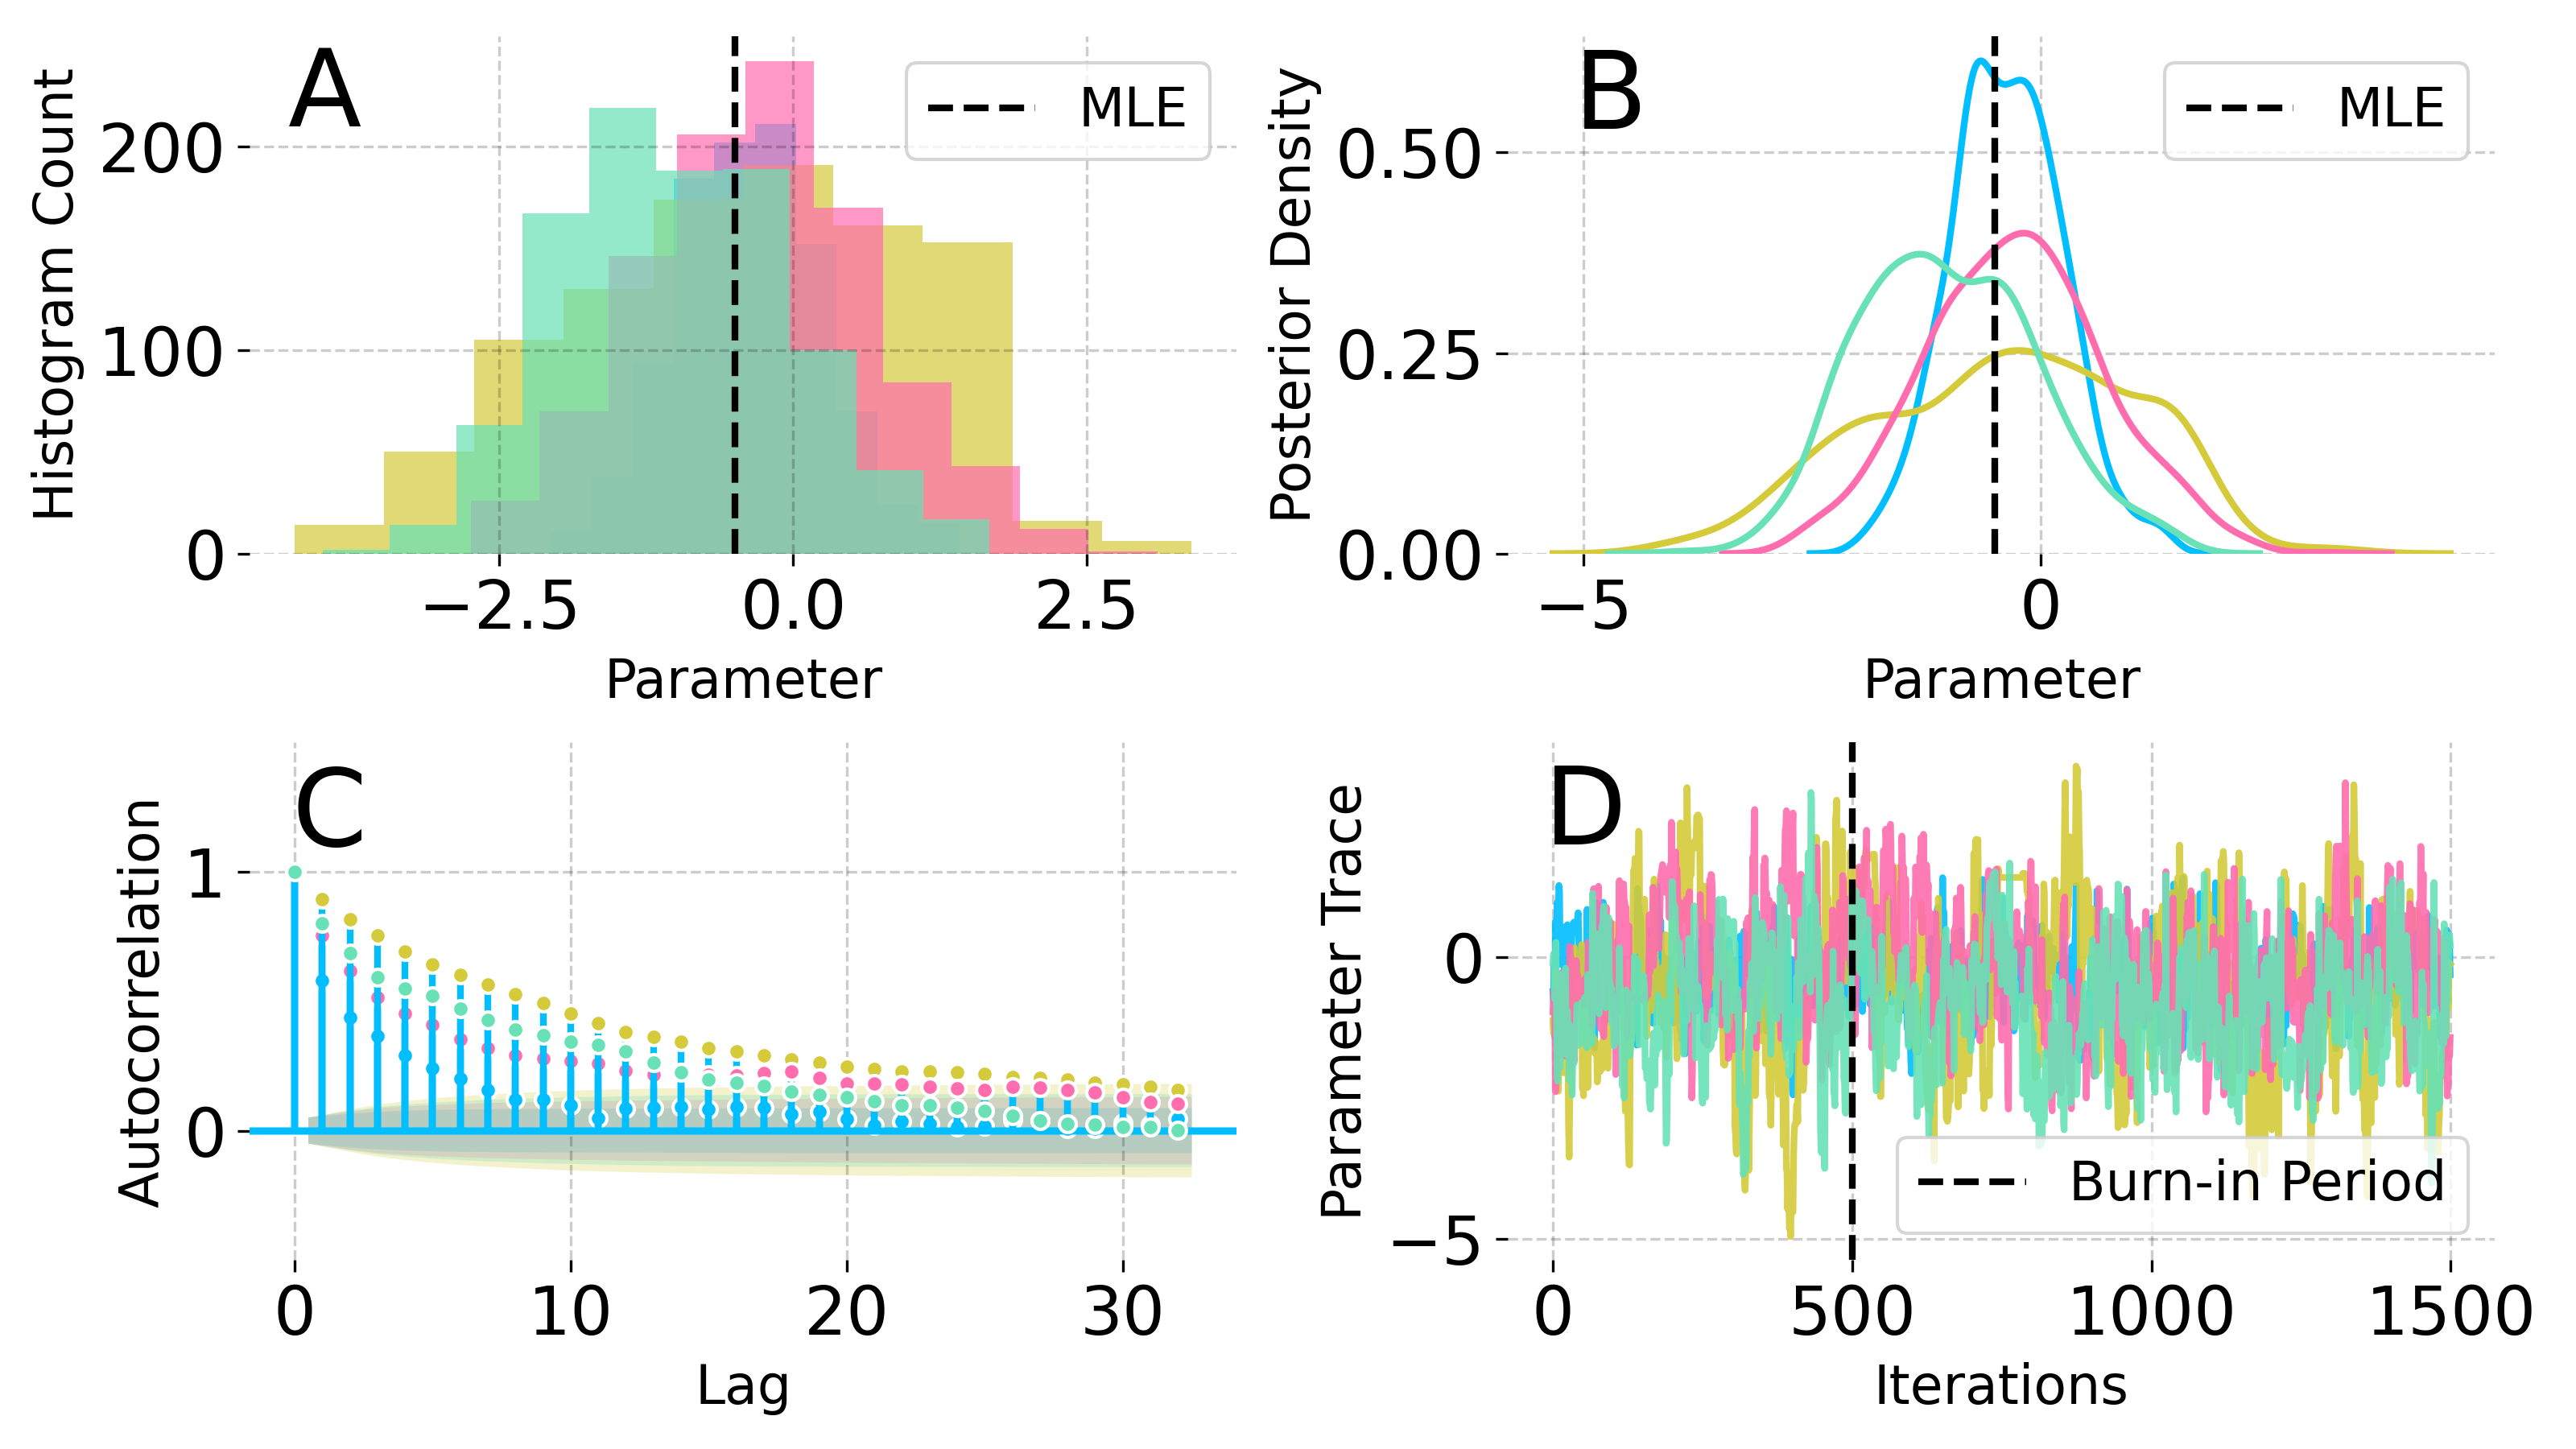
\includegraphics[width=\textwidth/\real{1.5}]{imgs/pmcmc/nuts_eb.png}
    \caption{Convergence diagnostics for a No U-Turn Sampler with the informative prior from IF2. The NUTS sampler mixes quickly, and the posterior estimates from each chain posterior modes.}
    \label{fig:nuts-eb}
\end{figure}

\end{frame}

\section{Conclusions and Future Work}

\begin{frame}{Conclusion}
    \begin{itemize}
        \item New theoretical framework/algorithm/gradient estimator that encompasses a few existing gradient estimates.
        \item \pause Promising hybrid algorithm that warm-starts gradient descent (using this estimator) with IF2.
        \item \pause Outperforms IF2 on Dhaka cholera model of \cite{king15}.
    \end{itemize}
\end{frame}


\begin{frame}{Future Work}
    \begin{itemize}
        \item MOP-$\alpha$ cannot handle discrete latent states. Maybe likelihood ratios can get around this.
        \item \pause Convergence rate of IF2 not known, conjecture similar behavior to SGD. 
        \item \pause Only gradient descent explored, other methods like Newton's method, ADAM, L-BFGS, etc. may perform better.
        \item \pause Extensions to panel and spatiotemporal data, e.g. with a block particle filter in the lens of \cite{ionides22} and \cite{ning23}.
        \item \pause Python counterpart to the popular \texttt{pomp} R package by \citet{king16, king2017pompmanual}.
    \end{itemize}
\end{frame}


\bibliographystyle{apalike}
\bibliography{paper/bib-ifad}


\end{document}

